
\begin{frame}{Praxis I}
Third International CSP Competition (CPAI’08)
\begin{center}
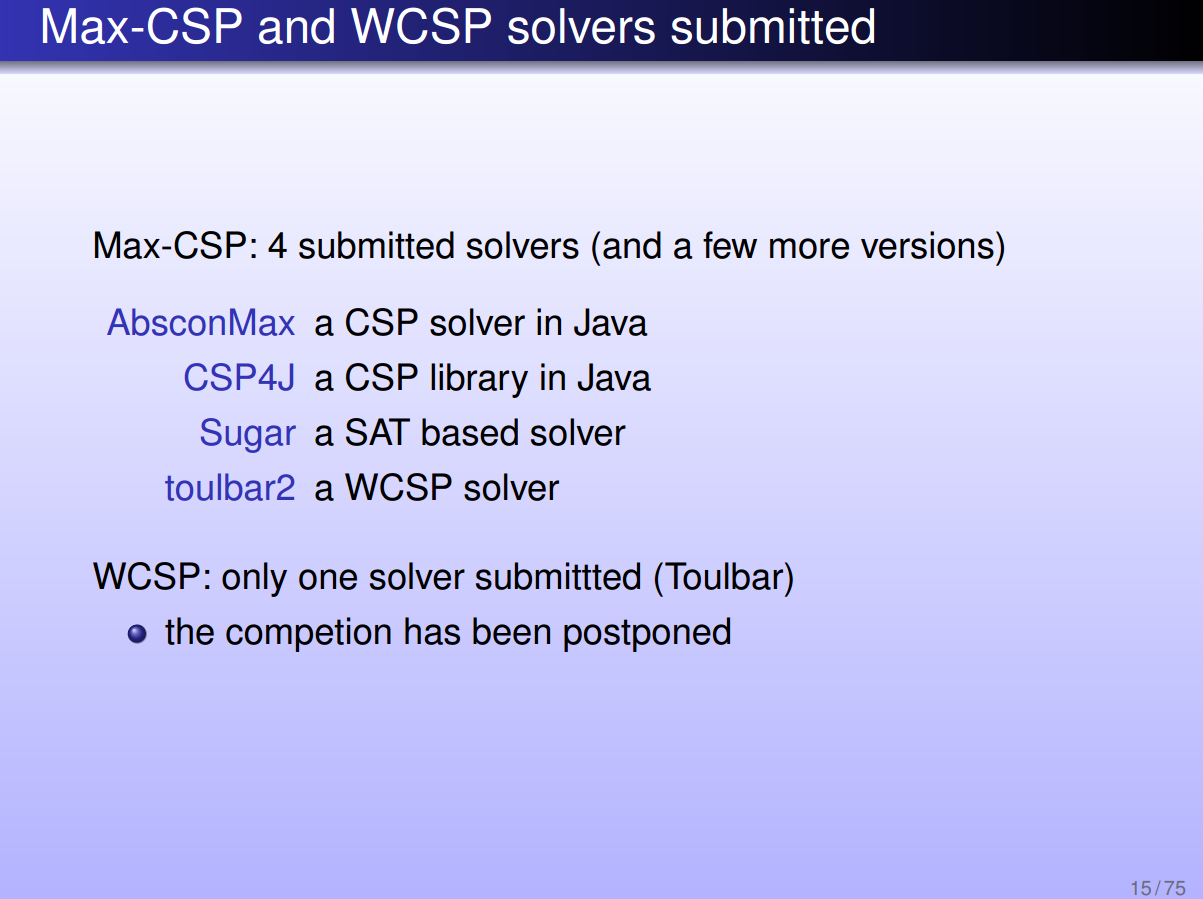
\includegraphics[width=.8\textwidth]{img/cpai08.png}
\end{center}
\end{frame}

\begin{frame}{Praxis II}
Im Constraint Programming:
\begin{itemize}
\item Fokus auf \emph{klassischen} Constraint-Lösern
\item Erweiterung auf einfache Optimierung (Branch \& Bound)
\item Zielfunktion kann skalare Variable (\texttt{int} oder \texttt{float}) sein
\item { \color{isseorange} \texttt{toulbar2} ist der einzige dedizierte Weighted-CSP-Solver}
\end{itemize}

\vspace*{2ex}

In der mathematischen Programmierung:

\begin{itemize}
\item Probleme müssen gewisse Struktur aufweisen (lineare Constraints, quadratische Constraints, etc.)
\item Schlecht geeignet für beliebige Ordnungen nach denen optimiert werden soll
\end{itemize}

\vspace*{1ex} \pause 
Wir wollen aber heterogene PVS $\rightarrow$ \alert{MiniZinc}
\end{frame}


\begin{frame}{Warum MiniZinc?}
\begin{parchment}[Rationale]
\centering 
\alert{Eine Modellierungssprache -- viele Solver} 
\end{parchment}

\begin{textblock*}{2.cm}[1,1](\textwidth-.5cm,\textheight-1.03cm)


\includegraphics[width=\textwidth]{img/MiniZn_logo.jpg} 

\end{textblock*}
\emph{Reduziere Soft-Constraint-Probleme auf konventionelle Constraint-Probleme}

\begin{itemize}
\item Gecode (CP)
\item JaCoP (CP)
\item Google Optimization Tools (CP)
\item CPLEX (CP/LP/MIP)
\item G12 (CP/LP/MIP)
\item \ldots
\end{itemize}
\end{frame}

\begin{frame}{MiniZinc-Challenge}
Findet jährlich seit 2008 statt. Klassische Constraint-Probleme in MiniZinc werden an teilnehmende Solver geschickt.

\begin{center}
Gewinner 2015

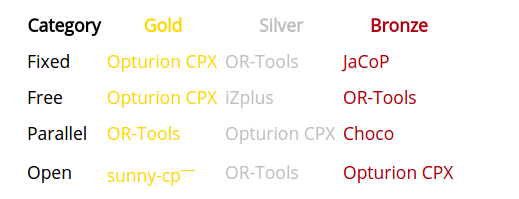
\includegraphics[width=.5\textwidth]{img/ergeb2015.png}


\end{center}
\begin{tabular}{|c|c|}
\hline 
Jahr & Teilnehmende Solver \\ 
\hline 
2015 & 20 \\ 
\hline 
2014 & 18 \\ 
\hline 
2013 & 10 \\ 
\hline 
2012 & 9 \\ 
\hline 
\end{tabular} 
\end{frame}